\documentclass{article}
\usepackage[paperwidth=9in,paperheight=4.6in,margin=0.12in]{geometry}
\usepackage{tikz}
\pagestyle{empty}
\begin{document}
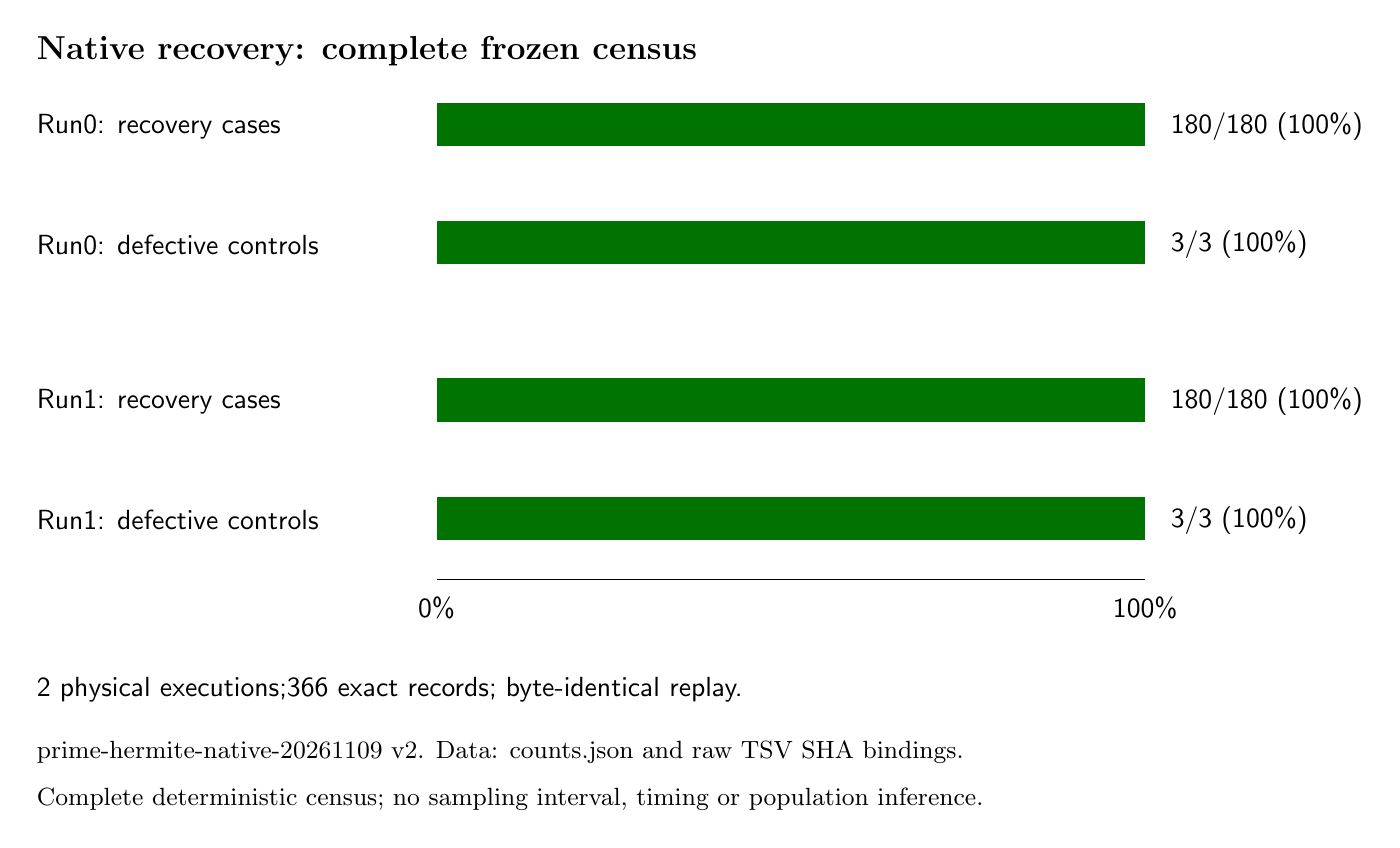
\begin{tikzpicture}[x=1cm,y=1cm,font=\sffamily]
\node[anchor=west,font=\large\bfseries] at(0,10){Native recovery: complete frozen census};
\foreach \y/\label/\count in {8.8/{Run0: recovery cases}/{180/180},7.3/{Run0: defective controls}/{3/3},5.3/{Run1: recovery cases}/{180/180},3.8/{Run1: defective controls}/{3/3}} {
 \node[anchor=west] at(0,\y+0.25){\label};
 \fill[green!45!black](5.2,\y) rectangle(14.2,\y+0.55);
 \node[anchor=west] at(14.4,\y+0.25){\count\ (100\%)};
}
\draw(5.2,3.3)--(14.2,3.3);
\node[anchor=north] at(5.2,3.2){0\%};\node[anchor=north] at(14.2,3.2){100\%};
\node[anchor=west] at(0,1.9){2 physical executions;366 exact records; byte-identical replay.};
\node[anchor=west,font=\small] at(0,1.1){prime-hermite-native-20261109 v2. Data: counts.json and raw TSV SHA bindings.};
\node[anchor=west,font=\small] at(0,0.5){Complete deterministic census; no sampling interval, timing or population inference.};
\end{tikzpicture}
\end{document}
